This section will explain how the model was trained, validated, and tested. Several adjustments were
made to improve the model's prediction accuracy. For the training process, the model was trained with
training data sets and validated with validation data sets. On the other hand, testing data sets are
completely different from the training and validation data sets.
The number of training data sets are 47930 and validation sets are 5325. The validation set size is
roughly 10 percent of the training data sets. Five different experiment took place to improve the
prediction accuracy. In order to see the difference in the experiment, the model was trained with two
different learning rate and the number of epochs; Learning rate was 0.0001 and 0.00001; The number of
epochs are 17, 21, and 27. Finally, one batch of data sets contain 32 data sets.
\newline
\newline
\indent
To begin with, during the training process, the goal is to minimize the validation loss. Therefore,
training with different independent variables such as epoch sizes and learning rates produced the various
accuracy when predicting. The training processes and the results of prediction with the prediction accuracy are
provided in the figures below. The size of increase in the number of iterations are limited in this experiemnt
because of the computational power limitation.
    \begin{figure}
        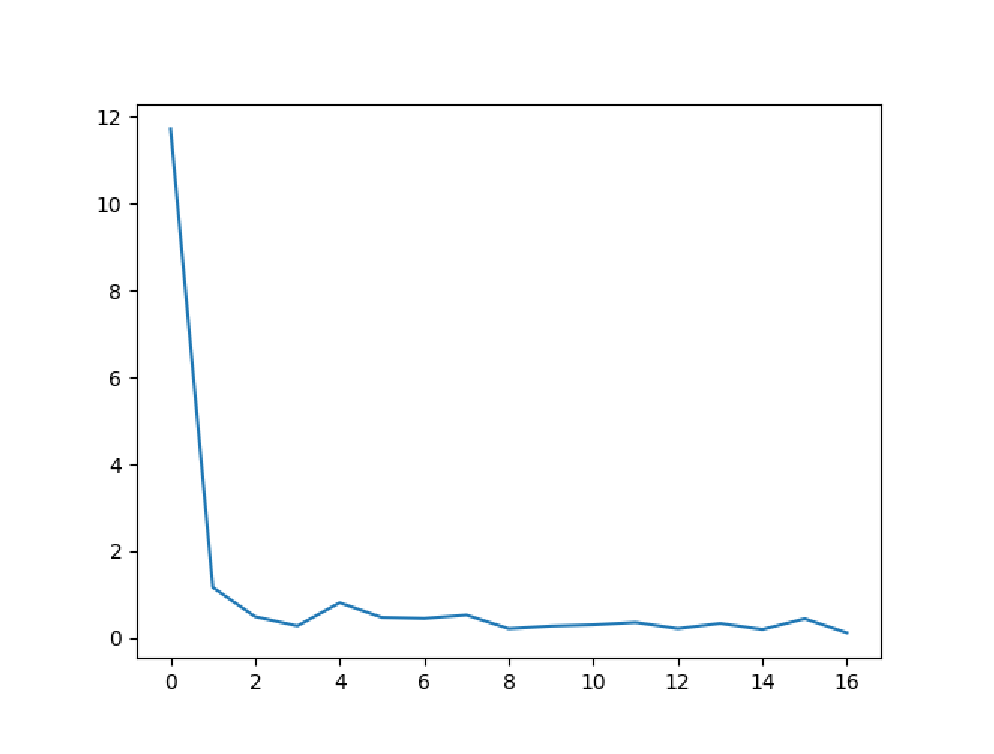
\includegraphics[width=\textwidth, scale=0.25]{4_25000.eps}
        \caption{Validation loss graph for epoch size 17 with learning rate 0.0001.} \label{Figure2}
    \end{figure}

    \begin{figure}
        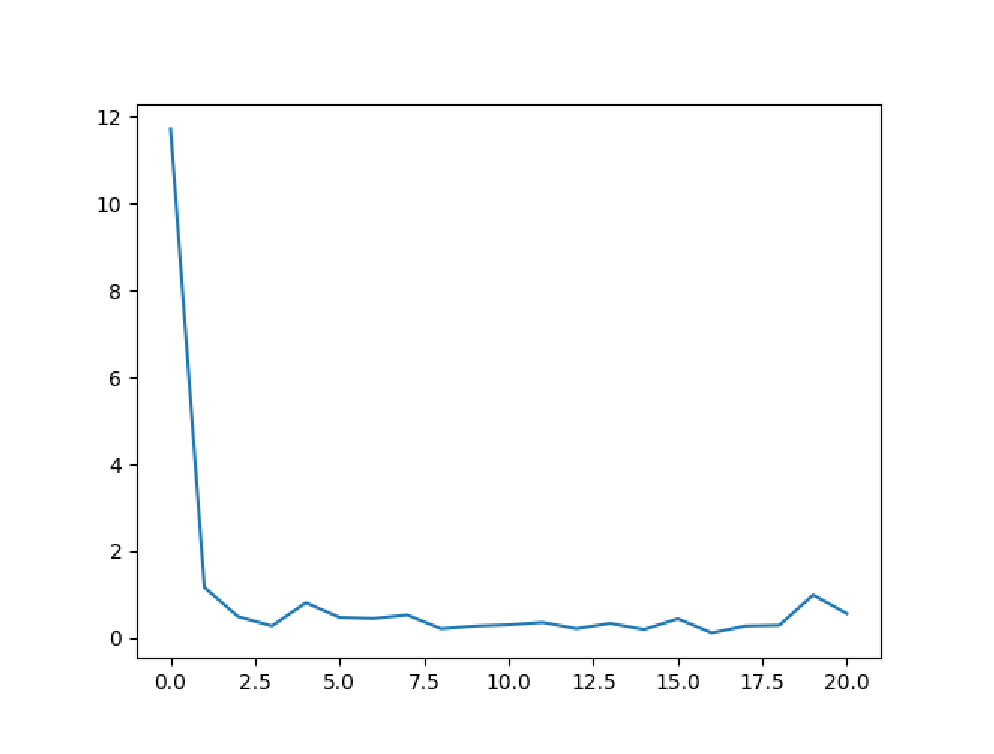
\includegraphics[width=\textwidth, scale=0.25]{4_30000.eps}
        \caption{Validation loss graph for epoch size 21 with learning rate 0.0001.} \label{Figure2}
    \end{figure}

    \begin{figure}
        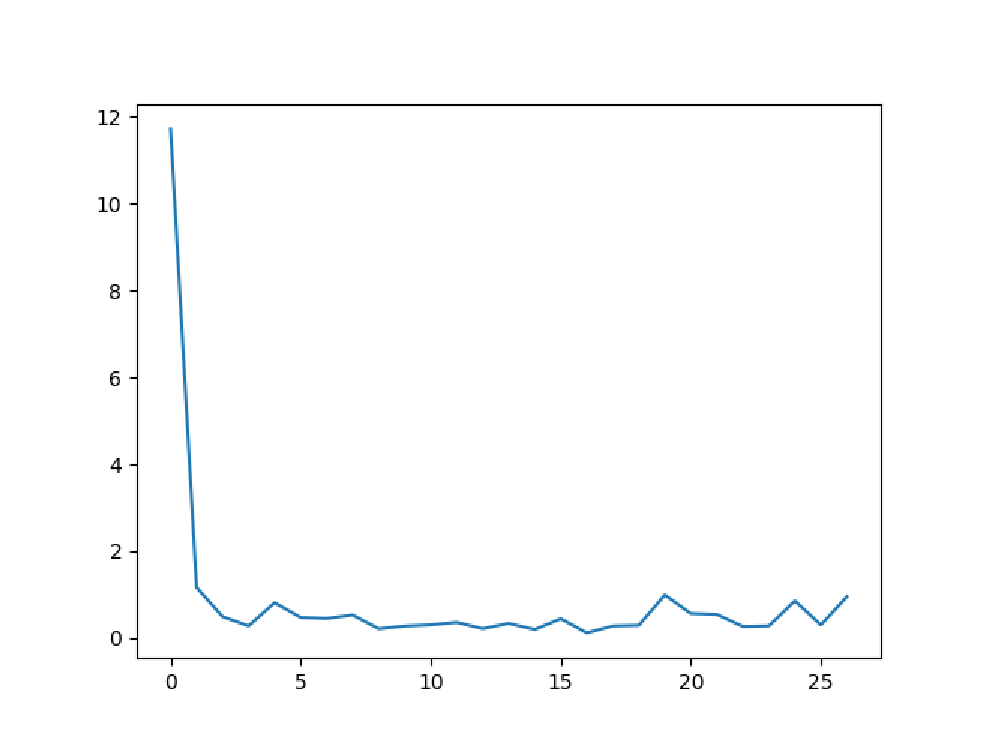
\includegraphics[width=\textwidth, scale=0.25]{4_40000.eps}
        \caption{Validation loss graph for epoch size 27 with learning rate 0.0001.} \label{Figure3}
    \end{figure}


    \begin{figure}
    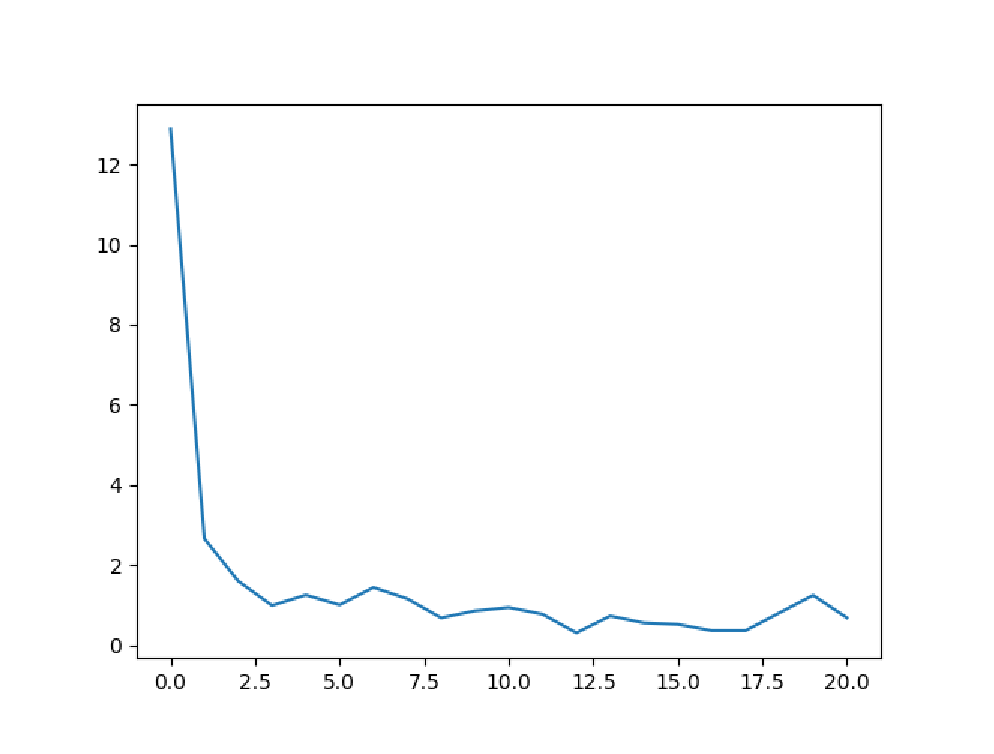
\includegraphics[width=\textwidth, scale=0.25]{5_30000.eps}
    \caption{Validation loss graph for epoch size 21 with learning rate 0.00001.} \label{Figure4}
    \end{figure}

    \begin{figure}
    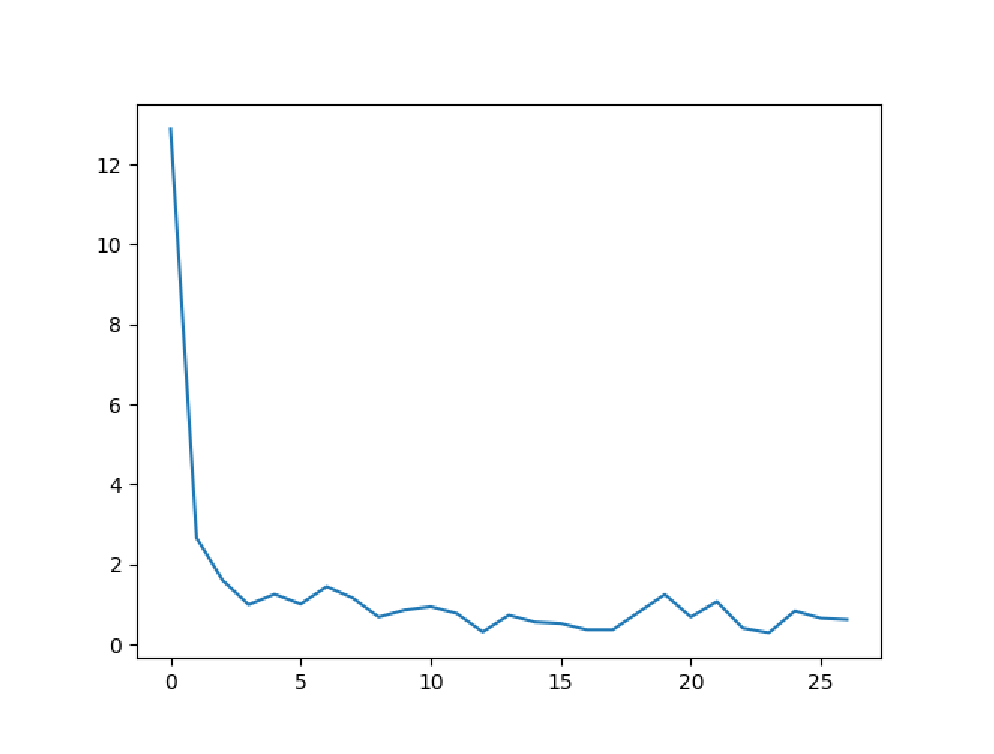
\includegraphics[width=\textwidth, scale=0.25]{5_40000.eps}
    \caption{Validation loss graph for epoch size 27 with learning rate 0.00001.} \label{Figure5}
    \end{figure}

Further explantion.